    \item The given  equations can be expressed as the matrix equation
    \begin{align}
\label{linform/11/cd/eq:1}
  \myvec{3&-5\\6&-10}\vec{x} &= \myvec{20\\40}
\end{align}
The augmented matrix for the above equation
is row reduced as follows
\begin{align}
    \myvec{3&-5&20\\6&-10&40}\xleftrightarrow{R_2\leftarrow R_2 -2R_1}\myvec{3&-5&20\\0&0&0} \label{linform/11/cd/eq:(2)}
\end{align}

Thus  \ref{linform/11/cd/eq:1} has infinitely many solutions and 
Fig. \ref{linform/11/cd/fig:1} shows that the lines are the same.
\begin{figure}[!ht]
    \centering
    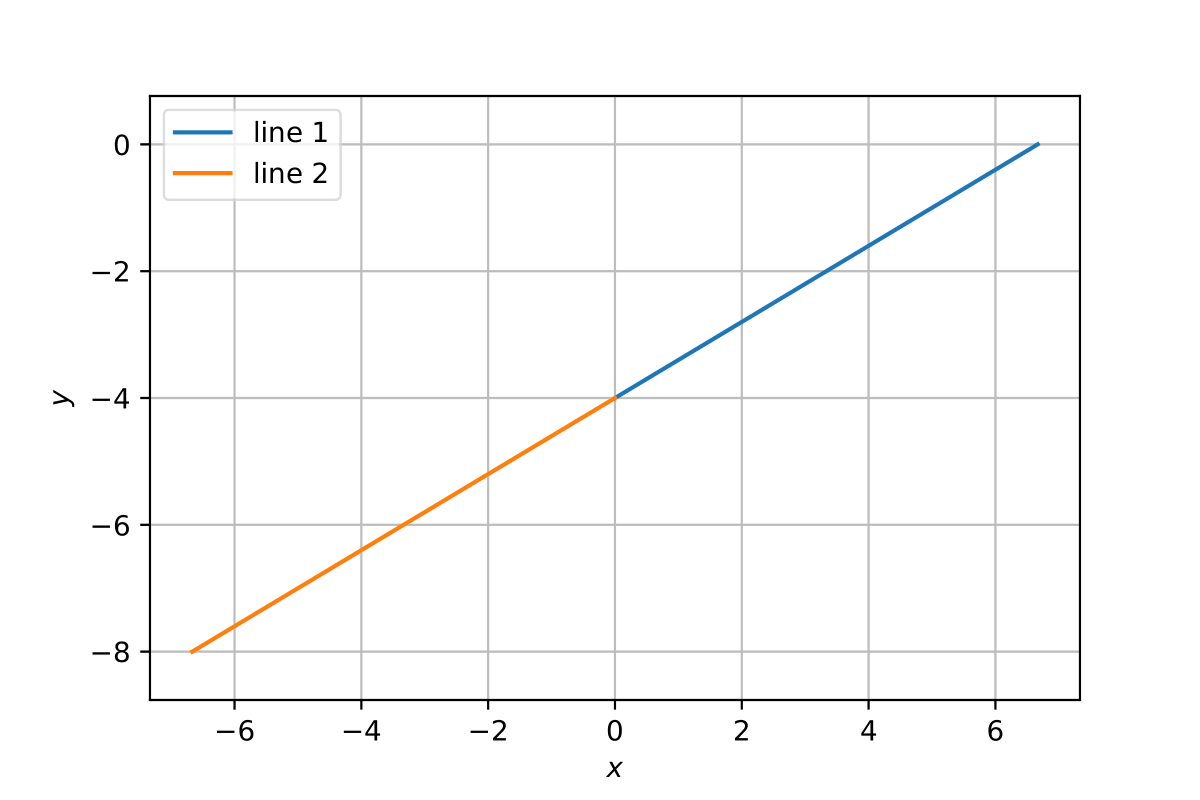
\includegraphics[width= \columnwidth]{solutions/su2021/2/11/cd/assignment2c-1.png}
    \caption{Lines coincide:infinitely many solutions}
    \label{linform/11/cd/fig:1}
\end{figure}
\item 
    The above equations can be expressed as the  matrix equation
    \begin{align}
\label{linform/11/cd/eq:7}
  \myvec{1&-3\\3&-3}\vec{x} &= \myvec{7\\15}
\end{align}
The augmented matrix for the above equation
is row reduced as follows
\begin{align}
    \myvec{1&-3&7\\3&-3&15}\xleftrightarrow{R_2\leftarrow R_2 -R_1}\myvec{1&-3&7\\2&0&8} 
    \\ 
    \myvec{1&-3&7\\2&0&8}\xleftrightarrow{R_2\leftarrow R_2 -2R_1}\myvec{1&-3&7\\0&6&-6} 
    \\
    \myvec{1&-3&7\\0&6&-6}\xleftrightarrow{R_1\leftarrow R_1 +\frac{R_2}{2}}\myvec{1&0&4\\0&6&-6} 
\\ \myvec{1&0&4\\0&6&-6}\xleftrightarrow{R_2\leftarrow\frac{R_2}{6}}\myvec{1&0&4\\0&1&-1} \label{linform/11/cd/eq:11}\end{align} 
\begin{align}
 \implies \vec{x}&=\myvec{4\\-1}
\end{align} is a solution of \ref{linform/11/cd/eq:7} which is verified through 
%
Fig. \ref{linform/11/cd/fig:2} 
%
\begin{figure}[!ht]
    \centering 
    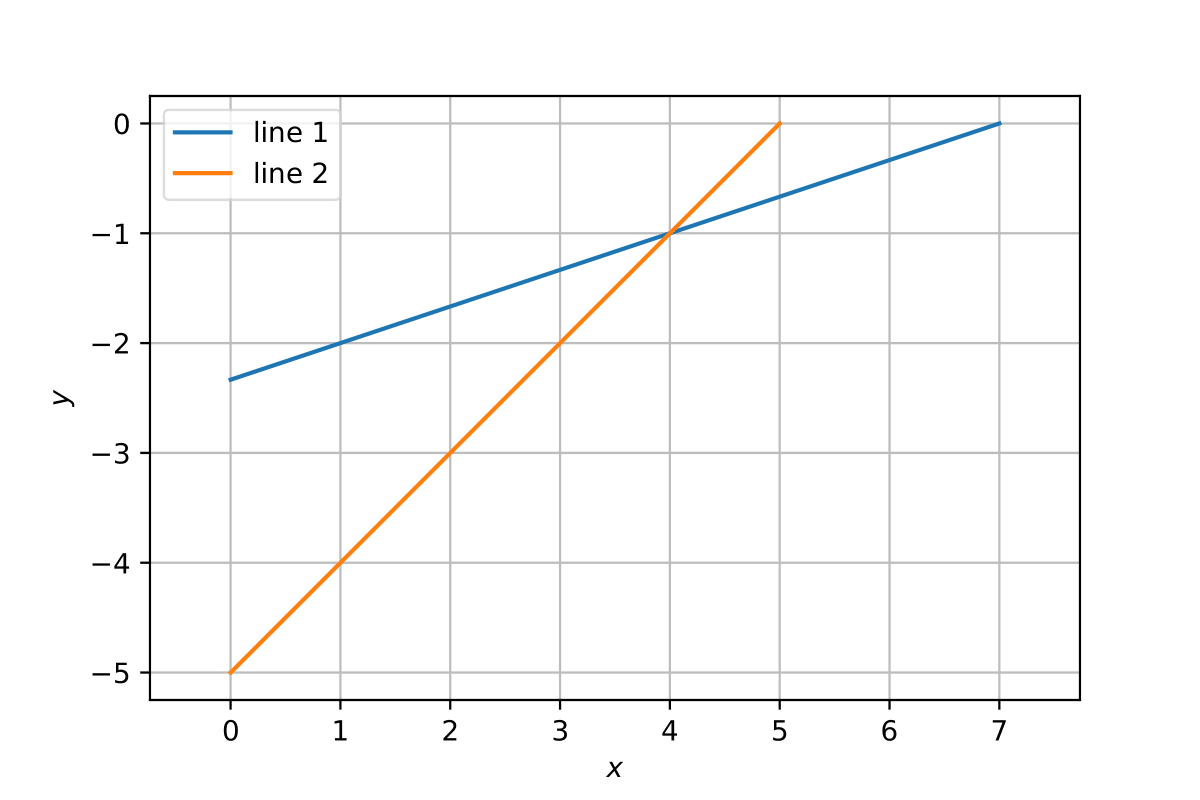
\includegraphics[width= \columnwidth]{solutions/su2021/2/11/cd/assignment2d-1.png}
    \caption{Lines intersecting only at one point:unique solution}
    \label{linform/11/cd/fig:2}
\end{figure}
